\section{System Overview}
\label{sec:overview}

Spider 2 which was deployed just before Spider 1 was retired in 2013 was
architected, deployed, and is operated by the OLCF staff; just as was done for
Spider 1. Figure~\ref{fig:arch} shows a conceptual architecture for Spider 2.
The primary building block is a DataDirect Networks SFA12KX RAID controller
pair (couplet) with 10 disk enclosures containing a total of 560 2TB NL-SAS disk drives.
8 Lustre OSS hosts are external to the SFA12KX and are connected to the couplet
via 2 FDR Infiniband links on each host for path redundancy. In total there are
36 building blocks that are build into two file system namespaces on
non-overlapping hardware resources (i.e. ``atlas1'' and ``atlas2''). The
resulting system was rated for, and tested to deliver an aggregate performance of 1.4 TB/s
for reads and 1.2 TB/s writes which translates into +1 TB/s aggregate read and
write performance at the file system level.

Table~\ref{table:spider12} highlights key characteristics of the Spider 1 and 2
file systems.

Through these deployments the OLCF has built comprehensive
monitoring tools for Spider\cite{ddntool10:ross}. Many of these monitoring
tools have been in-house developed at the OLCF, particularly the ``DDNTool'', a
tool which was developed for monitoring the I/O requests from at the DDN
controller level. With the release of SFAOS and the SFA Hardware platform, 
DDN created a python-based API for querying performance and request size data 
from their storage systems. ``DDNTool'' version 2 makes use of this API to query 
all 36 couplets for this data.


\begin{figure}[!t]
\centering
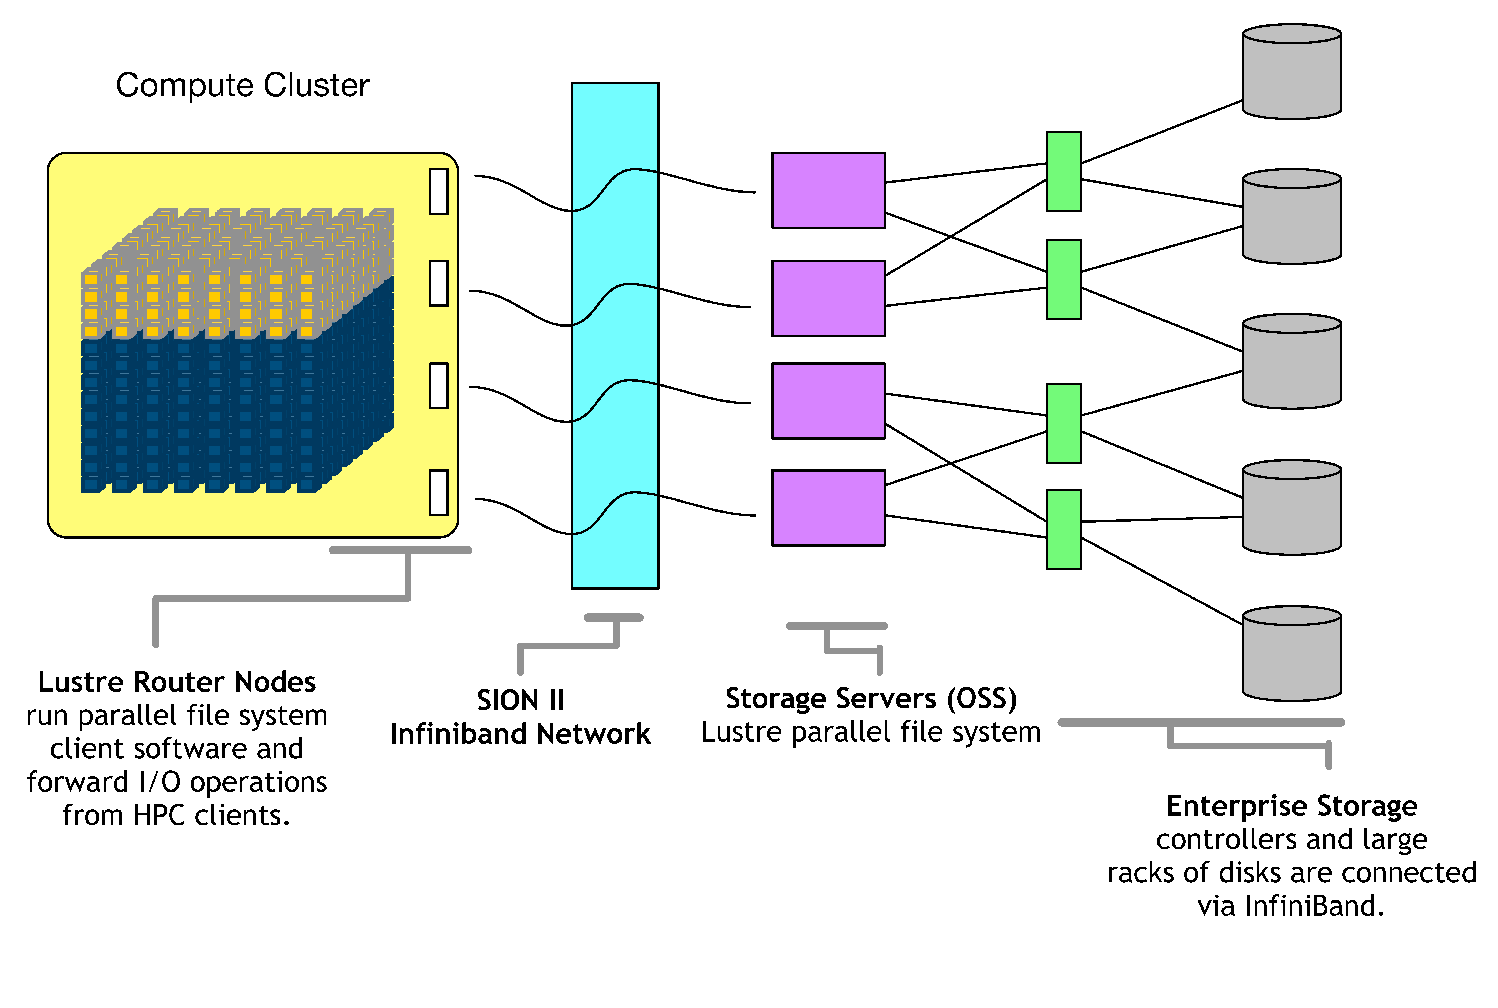
\includegraphics[width=0.45\textwidth]{./figs/spider2arch.ps}
\vspace{-0.1in}
\centering
\caption{Spider Architecture}
\label{fig:arch}
\end{figure}

\begin{table}
\begin{center}
\begin{tabular}{l||l|l}
 & Spider 1 & Spider 2\\
\hline
Bandwidth & 240 GB/s & +1 TB/s \\
Capacity & 10 PB & 32 PB \\
RAID Controllers & DDN S2A9900 & DDN SFA12KX\\
Disk type & SATA & Near-line SAS\\
Number of disks & 13,440 & 20,160\\
Disk redundancy & RAID 6 (8+2) & RAID 6 (8+2)\\
Number of OSTs & 1,344 & 2,016\\
Number of OSSs & 192 & 288\\
Lustre version & 1.8 & 2.5\\
Connectivity & IB DDR & IB FDR\\ 
\end{tabular}
\end{center}
\caption{Spider 1 and Spider 2 key specifications}
\label{table:spider12}
\end{table}


\subsection{Storage Controller Monitoring}

DDNTool \cite{ddntool10:ross} was developed to monitor the DDN S2A and SFA
storage system RAID controllers. Since the two DDN architectures have very
different monitoring API's, there are actually two completely separate
programs:  DDNTool for the S2A architecture and DDNTool\_v2 for the SFA
architecture.  The two tools are very different in their implementations -
DDNTool is a C++ program that communicates with the disk controllers directly
over TCP/IP while DDNTool\_v2 is a Python program that interfaces with a
vendor-supplied python library which handles the low level communication - but
they both accomplish the same basic task.  The tools poll each controller for
various pieces of information (e.g. I/O request sizes, write and read
bandwidths) at regular rates and store this information in a MySQL database.
The database is not actually used for long term storage.  In fact, at each poll
interval, the old data is overwritten with new data.  By storing a the data in
a database, though, the data is available to numerous clients via a
well-documented API.  This allows multiple users to search and query in
real-time.
